
\begin{figure}[htbp]
\renewcommand{\familydefault}{\sfdefault}\normalfont
\centering 
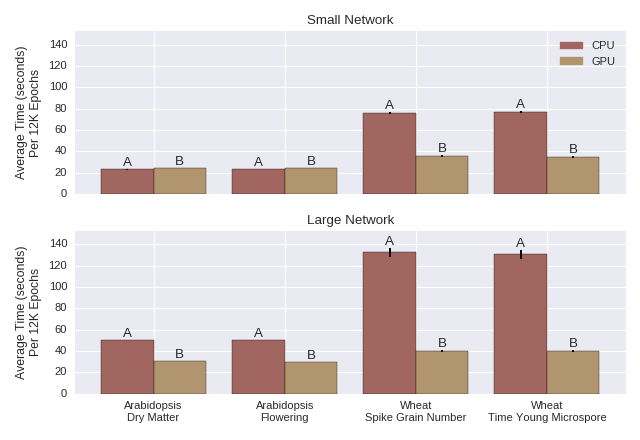
\includegraphics[width=\linewidth]{g3_article/figures/time_comparison.png}
    \caption{Time to train different sized networks on identical datsets using a single dedicated CPU core
             compared to a single dedicated GPU card. Lower time to train is better. For the small network, 
             an unregularized, single hidden layer of 27 neurons was trained for 12K epochs on each dataset. 
             For the large network, two the hidden layers of size 64 and 32 neurons, respectively were trained. 
             Training processes were otherwise equal. This process was repeated ten times per dataset to 
             reduce variation associated with non-deterministic processor scheduling and varying computer system load.
             The ten CPU and GPU training samples were compared using an independent samples T-test with $n=30$. 
             CPU-GPU pairs annotated with the same letter are not significantly different 
             at the $\alpha=0.05$ level.}
\label{fig:time-comparison}
\end{figure}
